\section{Technical algorithm details}
\label{sec:algorithm-details}
\setcounter{table}{0}
\renewcommand{\thetable}{A\arabic{table}}
\setcounter{figure}{0}
\renewcommand{\thefigure}{A\arabic{figure}}
\setcounter{algorithm}{0}
\renewcommand{\thealgorithm}{A\arabic{algorithm}}
\renewcommand{\theHalgorithm}{A.\arabic{algorithm}}

\subsection{Exact existence queries during growth}
\label{sec:existence-details}

An existence query takes the growing source fragment $F$, its accepted preservation edges $A$, and the assignments locked by completed fragments. Its output is one compatible injective assignment, or proof that none exists. It does not construct the completed fragment's alternative placements.

For each source atom $u$, a domain $D_u$ contains compatible target atoms. A locked atom has its recorded image as its only destination; other atoms exclude destinations occupied by completed fragments. Target degree must accommodate the accepted edges incident to $u$. For each accepted edge $(u,v)$, a support relation contains the target pairs satisfying the graph floor and matching tolerance. These are constraints on accepted edges only, without additional nonedge or induced-subgraph tests.

Propagation repeatedly removes occupied singleton destinations from other domains and removes any destination lacking support in a neighboring domain. An empty domain or conflicting singletons proves infeasibility. A bipartite matching check then tests whether the remaining domains admit distinct destinations for every source atom; it can reject competing domains without enumerating their assignments. These checks are necessary conditions. If choices remain, the solver selects the smallest domain, breaking ties by accepted-edge degree and atom index, and explores its destinations until the first solution is found. A negative answer requires exhaustion of the surviving choices. Difficult negative instances can therefore still require search.

A growth proposal first tries to reuse the previous witness: it already satisfies the earlier edges, so only the proposed edge and any newly joined locked atoms require checking. If that extension fails, earlier assignments within the growing fragment may change in a new exact query. Completed-fragment locks remain fixed. An interrupted query does not establish absence. The Python and native implementations follow these same rules; the native propagation tests bond support by scanning target neighbors against indexed domain membership.

\subsection{Direct compressed completion}
\label{sec:completion-details}

Completion starts from the finished fragment constraints. It partitions eligible target atoms into interchangeable classes: swapping two atoms within a class must preserve their eligibility, the relevant accepted-edge support relations, and the orbit, lock and policy context. For custom atom policies, compatibility with future source atoms is retained as well. Local interchangeability is a property of these matching predicates. Component labels alone do not split an otherwise interchangeable free-atom class.

The second equivalence is the exact global target automorphism action. Its colored graph retains the target's exact bond weights, edge presence, atom policy and component identities. Locks and current allocation roles further restrict this action. It can move atoms outside the fragment together with atoms inside it; individual orbit labels cannot replace these correlated moves. The automorphisms are obtained with nauty~\citep{mckay2014}.

The completion search allocates source atoms to target classes, rather than successively listing concrete bijections. After each allocation, the same support and injectivity propagation removes impossible continuations. Forced class choices are assigned directly. For an unresolved source atom, only one class representative from each orbit of the conditioned global action is explored. Conditioning preserves the allocations already made. A completed allocation yields a representative assignment, target pools and fixed roles; every represented injection within those pools satisfies the finished constraints. Pool allocations related by the allowed global action remain compressed. Thus distinct placements are constructed directly, without a subsequent candidate-merging pass.

\begin{algorithm}[t]
\caption{Separate fragment growth and completion}
\label{alg:fragment-details}
\small
\begin{algorithmic}[1]
\REQUIRE A seed, active source edges, completed-fragment locks and matching rules
\ENSURE Completed compressed placements and accepted/deferred edges
\STATE Initialize the growing fragment and one witness; return no placement if none exists
\STATE Initialize the accepted preservation edges
\WHILE{an eligible frontier proposal remains}
  \STATE Select a boundary atom and then an incident edge, each uniformly
  \STATE Form the proposed fragment, including a whole completed fragment if joined
  \STATE Retain the joined fragment's locked assignments and accepted preservation edges
  \STATE Extend the witness, or run the exact existence query with completed locks fixed
  \IF{a witness exists}
    \STATE Accept the selected edge and replace the growing witness
  \ELSIF{absence is proved}
    \STATE Defer the edge and continue with the remaining frontier
  \ENDIF
\ENDWHILE
\STATE Partition eligible target atoms by interchangeability for the finished constraints
\STATE Allocate source atoms to those classes using propagation and conditioned symmetry
\STATE Emit each distinct completed compressed placement once
\STATE Return placements to the reaction hierarchy for branching and cap checks
\end{algorithmic}
\end{algorithm}

\subsection{Conditional branches, caps and retained histories}
\label{sec:hierarchy-details}

Each completed placement produces a conditional continuation for later fragments. The cap counts compressed choices, not the bijections inside them, and applies both to an individual expansion and to the combined live continuations across parents. Exact continuation states may share a node while retaining all incoming histories. After these joins, a parent's new descendants are admitted together or rejected together if their addition exceeds the cap; descendants already joined to retained states remain represented. A capped expansion is not a partial list of the first $K$ placements and does not prove absence of other mappings.

The search retains every history reaching a live continuation or returned result. Mapping and boundary payloads with no surviving descendant are released, while compact cap records retain their context, attempted count, limit and number of occurrences. This storage sharing does not merge distinct mapping relations. Neither the branch cap nor the cache budget bounds every temporary allocation or total process memory.

\subsection{Finalization and conservative family reduction}
\label{sec:reduction-details}

Finalization supplies the saved symmetry actions needed to interpret each retained path. Family reduction then collects its terminal representative, required preservation edges, matching policy and ordered pool/group action program with earlier locks applied. It normalizes independent actions by commuting only those with disjoint support, and collapses identical adjacent full actions. Other overlapping actions retain their order.

Identical normalized records share one family. The public branch grouping uses the unordered collection of paired fragment atom sets, preserving the union of its family records, source histories and alternative fragment partitions. Equal witnesses, atom sets or automorphism groups alone do not establish family equality. This is conservative reduction of representations, not a semantic normal form proving that all remaining mapping sets are different or disjoint. It preserves the saved mapping union; it does not recover alternatives excluded by growth or caps.

\subsection{Local event responses and valid joint composition}
\label{sec:decoding-details}

The decoder first completes an inventory of fragment atom-set pairs and every use in the catalogue's families and alternative partitions. This shares structural descriptions. Shared event responses additionally require agreement of the local witness, relevant ordered actions and boundary context. Local action positions are bound back to the original family positions, so one action moving several fragments remains one joint choice.

For each relevant source pair, decoding follows its reachable target endpoint pairs under the ordered action program. Each group closes its pair orbit before the next action acts. For two distinct endpoints in a pool of size $k$, this involves at most $k(k-1)$ ordered pairs rather than $k!$ permutations. Before computing that orbit, the decoder tests a superset formed from the individual destination domains: if every pair has the same event response, that response is constant on the allowed choices too. A constant contribution avoids pair expansion but does not remove the underlying action or its constraints.

The local tables include source bonds, pairs that can reach a target bond, inter-fragment relationships and mapped/unmatched boundaries. Responses use the original endpoint weights and strict event thresholds. Target-side boundary contributions depend on which target atoms are occupied, without assigning correspondences to unmatched atoms. Constraints involving other atoms can restrict a pair projection, so the decoder validates the complete requested joint choice before combining local contributions. Each bond contributes once. Alternative partitions provide alternative decompositions of a family; their totals are not added.

\begin{algorithm}[t]
\caption{Prepare local responses and evaluate a requested family choice}
\label{alg:decoding-details}
\small
\begin{algorithmic}[1]
\REQUIRE A reduced catalogue and original endpoint matrices
\STATE Inventory all unique fragments, occurrences, partitions, actions and boundaries
\STATE Build shared internal-fragment and boundary response tables
\STATE Retain the family bindings and constraints connecting those tables
\FORALL{requested joint choices}
  \STATE Validate the saved ordered actions, injectivity and preservation constraints
  \STATE Choose one saved fragment partition of the family
  \STATE Combine its internal and boundary responses, counting each bond once
  \STATE Return event counts and, when requested, the corresponding bond changes
\ENDFOR
\end{algorithmic}
\end{algorithm}

This preparation neither rematches fragments nor enumerates complete bijections. Pair tables can still grow with the reachable domains. Ordinary decoding also does not enumerate unique whole-reaction event classes or choose a minimum-event mapping; the archived event-window study below used a separate explicit query.

\subsection{Completed-fragment reuse}
\label{sec:cache-details}

The cache stores completed compressed fragment results and the dependencies read during growth and completion. A reuse request must agree on the endpoint problem, matching rules, seed/random settings, branch settings and target occupancy. It then checks the assignments and completed-fragment memberships actually consulted, topology reads affected by changed cuts, and relevant deferred boundaries. Changes outside those dependencies can reuse the result; a changed relevant lock cannot. Unaffected external deferred edges are carried forward with the reused result.

Retention is bounded and oversized entries need not be cached. Eviction changes computation, not the returned placements or cap decisions. Shared snapshots carry endpoint, policy and code identity with integrity checks. At task boundaries a worker can load the latest compatible snapshot; an immutable first snapshot remains available if the latest stored version cannot be loaded. Publication replaces complete snapshots atomically. This is recovery of reusable data, not a different matching algorithm. Scheduling and storage do not alter the scientific search conditions.

\section{Reproducibility}
\label{sec:reproducibility}

The repository's \texttt{manuscript/REPRODUCIBILITY.md} links the benchmark scripts, pinned software and input versions, full configurations, and per-case records. It distinguishes the completed Golden validation in \Cref{sec:current-validation} from the archived September evaluations below. \Cref{tab:protocol} gives the archived comparison settings. The guide \texttt{docs/PYTHON\_API.md} demonstrates matching, family reduction, separate local decoding and conditional symmetry queries through the Python API.

The current Golden validation used source \texttt{096a010961f53944ddd4ddc433bd8d56f282a2f2}, with fresh results and caches. The current main-text timing figure sums total task-worker CPU, including computation and result publication, across both directions and all four stages, then divides by 1,851 reactions. Its mean is 10.01 CPU seconds per reaction. Coordinator activity, startup and idle capacity are excluded; this is not elapsed latency. Compute-only CPU is recorded separately and excludes publication. The current evidence does not record a CPU model, so these measurements do not establish a hardware-normalized comparison. They are not pooled with the historical timing cohorts.

The WBO-generation method for the archived coordinate inputs is not recorded in the available metadata, so regeneration of those matrices from molecular structures is not established.

The archived paired search timings use an Apple M4 Pro CPU. Averages use \CommonCases{} common completed reactions. Reference verification and interrupted work are excluded. MAPPA includes checkpoint I/O; SLAP excludes I/O. Higher-seed runs measured on different CPUs are excluded from this paired comparison. For the archived coordinate stage comparison, MAPPA search includes checkpoint I/O; SLAP mapping excludes input preparation and export, and its hydrogen refinement includes I/O. Shared event rescoring and failed or replaced attempts are excluded. Archived Golden MAPPA timing includes symmetry finalization; SLAP includes graph construction, mapping, and export. In that primary Golden evaluation, uncut and swept SLAP have one and three unresolved cases, respectively; all MAPPA verdicts are resolved. These timing cohorts are not pooled with the current-design validation.

\section{Archived September evaluations}
\label{sec:historical-evaluation}

The following studies used their recorded September implementations. They retain the original numerical results and comparison scopes; they are not reruns of the current algorithm or direct performance comparisons with \Cref{sec:current-validation}.

\subsection{Archived datasets and comparator protocol}
\label{sec:default-comparators}

Golden inputs use formal bond orders and explicit H, with reference labels removed before search. Recovery requires the annotated heavy-atom correspondence, including unmatched atoms, modulo endpoint chemical symmetries preserving charge, isotope, H count, and stereochemistry. These chemical colors define reference equivalence; they do not imply that element/WBO matching itself enforces every chemical attribute. Failures and unresolved cases remain in the denominator. This measures reference inclusion among returned alternatives, not their ranking.

LocalMapper provides the prior accuracy-SOTA baseline~\citep{chen2024}. Its published Golden accuracy was 89.8\% on 1,758 retained reactions with manual calibration. SLAP reported 86.9\% on that dataset version, counting reference inclusion among its candidates~\citep{koda2025}. These literature scores are separate from our strict re-evaluation. We additionally apply the cut sweep introduced here to SLAP; ``SLAP sweep'' denotes this extension, not a published SLAP score. It is our strongest evaluated prior-method baseline for alternative recovery. Released RXNMapper, Chython, Indigo, and RDT provide further comparisons~\citep{schwaller2021,chython,indigo,rahman2016}.

The coordinate collection contains 18--137 explicit atoms per endpoint, including organometallic and multicomponent structures. It was inspected during development and has no verified atom mappings: it is not a mapping-accuracy benchmark. The archived study compared the lowest event count found and the patterns achieving that count. MAPPA used supplied WBO matrices; SLAP used XYZ-derived binary graphs. Returned SLAP heavy-atom assignments received hydrogen refinement and were scored on the same WBO matrices as MAPPA. The comparison covers those saved witnesses, not all possible SLAP hydrogen assignments or a fresh current-implementation evaluation.

Released comparators received the same label-free Golden inputs, without prediction repair or reference-guided ranking. Invalid endpoint chemistry, duplicate atom labels and other failures remained in the denominator. Binary SLAP was retained as the stronger default configuration; bidirectional comparisons used both binary and weighted modes. SLAP returns multiple candidates, whereas the other comparators return at most one explicit bijection. These results describe the evaluated interfaces and scoring rule, including its difference from RDT's chemical-change criterion. The repository records released models, versions, adapter settings and failure frequencies.

\subsection{Archived evaluation configurations}

\begin{table}[tb]
\centering\small
\caption{\textbf{Archived evaluation configurations.} Both use $b=0.2$, $\tau_{\mathrm{iso}}=1$, explicit H, and uncut plus single-edge searches. One seed per cut and the sweep define the default setting. Archived Golden measurements cover sweep search; no-sweep controls retain only the uncut graph. A seed setting counts source-atom orderings per cut.}
\label{tab:protocol}
\begin{tabular}{lcc}\toprule
Setting & Golden & Coordinate/WBO\\\midrule
Reactions & 1,851 & 140\\
Search directions & Bidirectional & Reactant to product\\
Seed orderings & 1 (default), 2, 3, 10 & 1 (default)\\
Branch cap & 100 (default) & 100 (default), 2,000\\
Evaluation & Reference-family recovery & Signed event-class coverage\\\bottomrule
\end{tabular}
\end{table}

\Cref{tab:protocol} lists the archived settings. Search did not use reference or comparator correspondences. Full configurations, implementation versions, and reproduction scripts are provided in the repository (\Cref{sec:reproducibility}).

\subsection{Archived Golden reference recovery and search cost}

In the archived campaign, the one-seed MAPPA configuration recovered \GoldenOnePercent\% of Golden references, compared with \SlapPercent\% for SLAP sweep (\Cref{tab:competitors,fig:golden}). These scores belong to that campaign, separate from \Cref{sec:current-validation}. The paired comparison includes \AamOnly{} references recovered only by MAPPA and \SlapOnly{} only by SLAP. LocalMapper is the strongest evaluated method returning one bijection. Additional MAPPA seeds yielded modest recovery gains at increasing search cost; two seeds did not improve recovery over one.

\begin{table}[tb]
\centering\small
\setlength{\tabcolsep}{4pt}
\caption{\textbf{Golden reference recovery and runtime in the archived evaluation.} Recovery uses all 1,851 primary-evaluation records. MAPPA retains compressed families; SLAP returns explicit candidates; other methods return one bijection over their matched atoms. MAPPA uses cap 100 and bidirectional search. Bidirectional SLAP combines both directions and both binary/weighted modes; the default SLAP row uses binary only. Times are mean CPU seconds per reaction, excluding separate bond-event decoding. Unmarked times use the same 1,403 completed reactions on an AMD EPYC 9J14. $a$: archived completed calls (1,718--1,851 per method), CPU model unrecorded; these times are not directly comparable with unmarked times. $\dagger$: LocalMapper, prior accuracy SOTA (2024). $\ddagger$: SLAP with our sweep, strongest evaluated prior-method recovery baseline.}
\label{tab:competitors}
\begin{tabular}{@{}lllr r@{}}\toprule
Method & Search setting & Output & Reference recovered & Mean CPU s\\\midrule
MAPPA & 1 seed, sweep (default) & Families & 1,834 (99.08\%) & 0.963 \\
MAPPA & 2 seeds, sweep & Families & 1,834 (99.08\%) & 1.619 \\
MAPPA & 3 seeds, sweep & Families & 1,837 (99.24\%) & 2.265 \\
MAPPA & 10 seeds, sweep & Families & 1,840 (99.41\%) & 6.993 \\
MAPPA & 1 seed, no sweep & Families & 1,489 (80.44\%) & 0.040 \\
SLAP, bidirectional & No sweep & Candidates & 1,661 (89.74\%) & 0.105 \\
SLAP, bidirectional$^{\ddagger}$ & Sweep & Candidates & 1,796 (97.03\%) & 2.793 \\
SLAP, binary & Default, no sweep & Candidates & 1,591 (85.95\%) & 0.075$^{a}$ \\
RXNMapper & Default, no sweep & One bijection & 1,547 (83.58\%) & 0.056$^{a}$ \\
LocalMapper$^{\dagger}$ & Default, no sweep & One bijection & 1,605 (86.71\%) & 0.294$^{a}$ \\
Chython & Default, no sweep & One bijection & 1,561 (84.33\%) & 0.612$^{a}$ \\
Indigo & Default, no sweep & One bijection & 692 (37.39\%) & 0.184$^{a}$ \\
RDT & Default, no sweep & One bijection & 1,030 (55.65\%) & 1.021$^{a}$ \\
\bottomrule\end{tabular}

\end{table}

The paired archived controls attribute 345 additional reference recoveries to the MAPPA sweep and 135 to the SLAP sweep. Without the sweep, one-seed MAPPA had lower coverage than bidirectional SLAP. This supports varying the growth constraints to expose alternatives excluded by greedy fragment extension (\Cref{sec:cut-sweep}); symmetry expansion alone cannot restore discarded placements. These differences are not measurements of a current no-sweep control.

Smaller-first grows fragments from the reaction side with fewer explicit atoms (including H) and matches into the other side; larger-first reverses these roles. In the archived comparison, combining both directions added 31 recoveries over smaller-first alone, demonstrating complementary alternatives (\Cref{tab:directions}).

\begin{table}[tb]
\centering\small
\caption{\textbf{Archived recovery and runtime by search orientation.} All rows use the sweep. Recovery uses all 1,851 Golden records; CPU statistics are seconds per reaction over the same \CommonCases{} completed reactions (Apple M4 Pro CPU). Smaller-first grows from the side with fewer explicit atoms, including H; larger-first reverses the source and target. Equal-size ties use stored order and its reverse. Bidirectional output combines both searches, and its CPU cost is their sum. SLAP combines binary and weighted modes. CPU/SLAP compares means within each orientation. Timing scopes are specified in \Cref{sec:reproducibility}.}
\label{tab:directions}
\begin{tabular}{@{}llrrrrr@{}}\toprule
Method & Orientation & Recovered & Mean & Median & 95th pct. & CPU/SLAP\\\midrule
MAPPA, 1 seed (default) & Smaller-first & 1,803 (97.41\%) & 1.141 & 0.263 & 5.289 & 0.34\\
 & Larger-first & 1,779 (96.11\%) & 1.377 & 0.348 & 6.401 & 0.92\\
 & Bidirectional & 1,834 (99.08\%) & 2.518 & 0.719 & 12.913 & 0.52\\
\midrule
MAPPA, 2 seeds & Smaller-first & 1,815 (98.06\%) & 2.232 & 0.416 & 10.635 & 0.67\\
 & Larger-first & 1,805 (97.51\%) & 2.721 & 0.578 & 14.064 & 1.83\\
 & Bidirectional & 1,834 (99.08\%) & 4.953 & 1.250 & 26.350 & 1.03\\
\midrule
SLAP sweep (prior baseline) & Smaller-first & 1,775 (95.89\%) & 3.329 & 0.422 & 4.752 & 1.00\\
 & Larger-first & 1,770 (95.62\%) & 1.490 & 0.455 & 4.568 & 1.00\\
 & Bidirectional & 1,796 (97.03\%) & 4.819 & 0.881 & 11.048 & 1.00\\
\bottomrule\end{tabular}

\end{table}

In these archived measurements, one-seed MAPPA had a lower mean and median search cost than SLAP sweep, but a higher 95th percentile. Two seeds approximately doubled the mean cost without improving recovery. These Golden timings cover search, excluding reference verification and separate bond-event decoding. The two timing tables use different experiments and should be compared within their stated CPU and reaction sets; neither establishes a current-implementation speed ranking.

In the archived cap study, increasing the branch cap from 100 to 2,000 yielded no additional swept recoveries among cases resolved at both caps, while increasing cost and unresolved outcomes at higher seed counts (\Cref{tab:golden-caps}). The uncut search gained 19 confirmed recoveries. Thus, in that study a larger branch budget did not substitute for changing the growth conditions.

\begin{figure}[tb]
\centering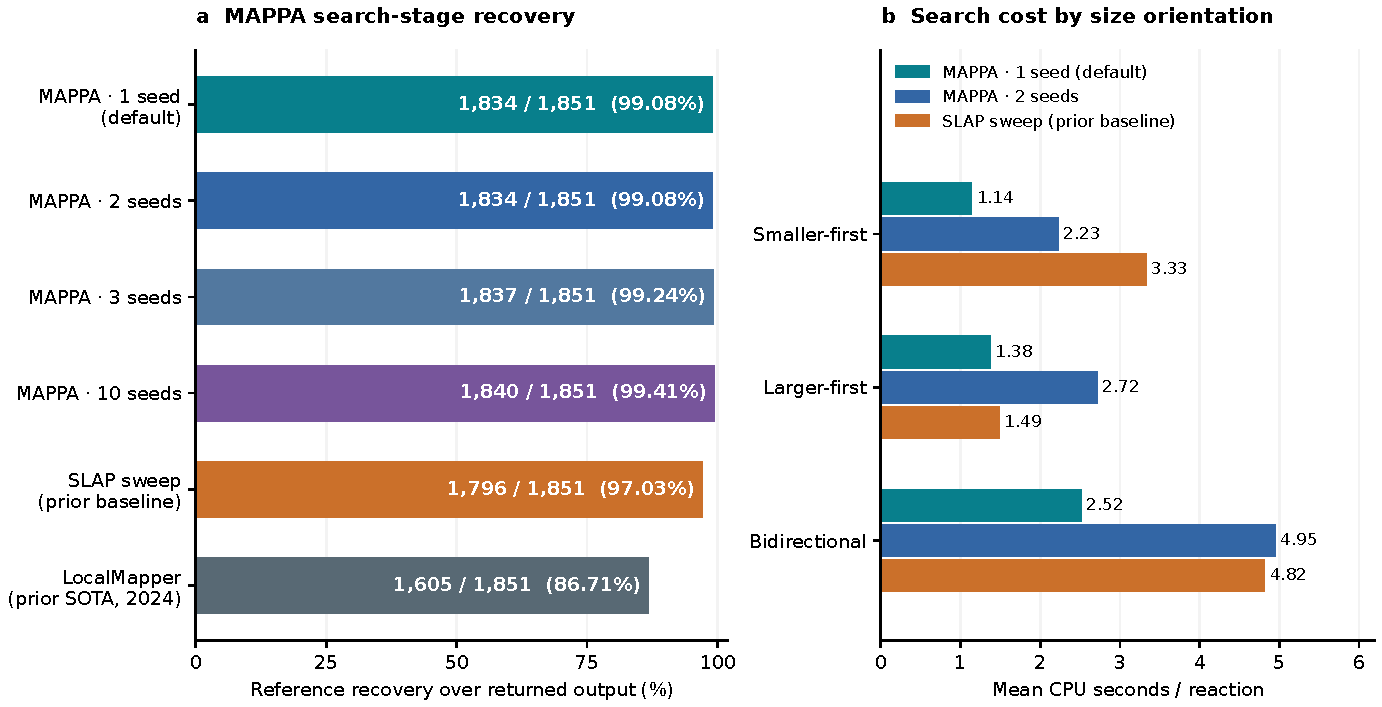
\includegraphics[width=\linewidth]{figs/fig2_golden.pdf}
\caption{\textbf{Archived Golden reference recovery and search cost.} (a) Reference recovery over all 1,851 reactions. MAPPA and SLAP use our cut sweep; LocalMapper is the prior accuracy-SOTA baseline and returns one bijection. All scores use the archived evaluator. (b) Mean search CPU over the same \CommonCases{} completed reactions, by orientation. Bond-event decoding is excluded. Full comparisons and timing scopes are in \Cref{tab:competitors,tab:directions}.}
\label{fig:golden}
\end{figure}

\FloatBarrier
\subsection{Archived bond-event comparison on 140 coordinate reactions}

The archived coordinate study used one-seed MAPPA sweep search with a branch cap of 2,000 and returned complete mappings for all 140 reactions. At cap 100, cases 123 and 125 returned no complete mapping. The 2,000-branch configuration therefore supplies this comparison, while 100 remains the library default. These completion counts and the event-window results below have not been remeasured with the current implementation.

The archived MAPPA output matched or lowered the minimum event count found by both native SLAP and SLAP sweep in every reaction (\Cref{tab:coordinate-minima,fig:coordinate}). This does not imply recovery of every alternative: at equal minima, six SLAP-sweep patterns remained absent across four reactions. An equal count can describe different changed bonds, and a lower count alone does not establish a more plausible transformation.

\begin{table}[H]
\centering\small
\caption{\textbf{Archived minimum bond-event comparison on 140 reactions.} MAPPA uses one-seed sweep search at cap 2,000. The first three columns count reactions by MAPPA's minimum event count relative to the comparator. The final column gives comparator minimum-event patterns recovered by MAPPA among reactions with equal minima. Counts refer to returned candidates, not proven global optima.}
\label{tab:coordinate-minima}
\begin{tabular}{@{}lrrrr@{}}\toprule
Compared with & MAPPA fewer & Equal & MAPPA more & Patterns at equal minima\\\midrule
SLAP sweep & 4 & 136 & 0 & 158/164\\
Native SLAP & 15 & 125 & 0 & 138/140\\
\bottomrule\end{tabular}

\end{table}

To compare alternatives above MAPPA's own minima, the archived study queried through one event above the higher of the two SLAP minima for each reaction. MAPPA retained 162 of 168 SLAP-sweep minimum-event patterns and 151 of 160 native-SLAP patterns within these windows. The output contains 300 distinct patterns, including 166 at MAPPA's own minima. Every saved family was exhausted or certified within its window; this establishes completeness for those retained families, not exhaustive structural search.

\begin{table}[H]
\centering\small
\caption{\textbf{Archived stage CPU time per reaction on the 140 coordinate reactions.} Measurements use an Apple M4 Pro CPU. MAPPA uses one-seed sweep search at cap 2,000. These stage costs exclude MAPPA decoding and do not establish an end-to-end speed ranking. SLAP refinement covers its returned witnesses. Timing boundaries are specified in \Cref{sec:reproducibility}.}
\label{tab:coordinate-time}
\begin{tabular}{@{}lrrr@{}}\toprule
Recorded stage & Mean CPU s & Median CPU s & 95th pct. CPU s\\\midrule
MAPPA sweep search & 1.047 & 0.314 & 3.481\\
SLAP sweep mapping & 1.337 & 0.546 & 5.919\\
SLAP H refinement / initial scoring & 0.053 & 0.011 & 0.207\\
\bottomrule\end{tabular}

\end{table}

The stage timings in \Cref{tab:coordinate-time} cover different outputs: MAPPA search retains families for subsequent decoding, while SLAP refinement operates on returned witnesses. They therefore do not establish an end-to-end speed ranking.

\begin{figure}[tb]
\centering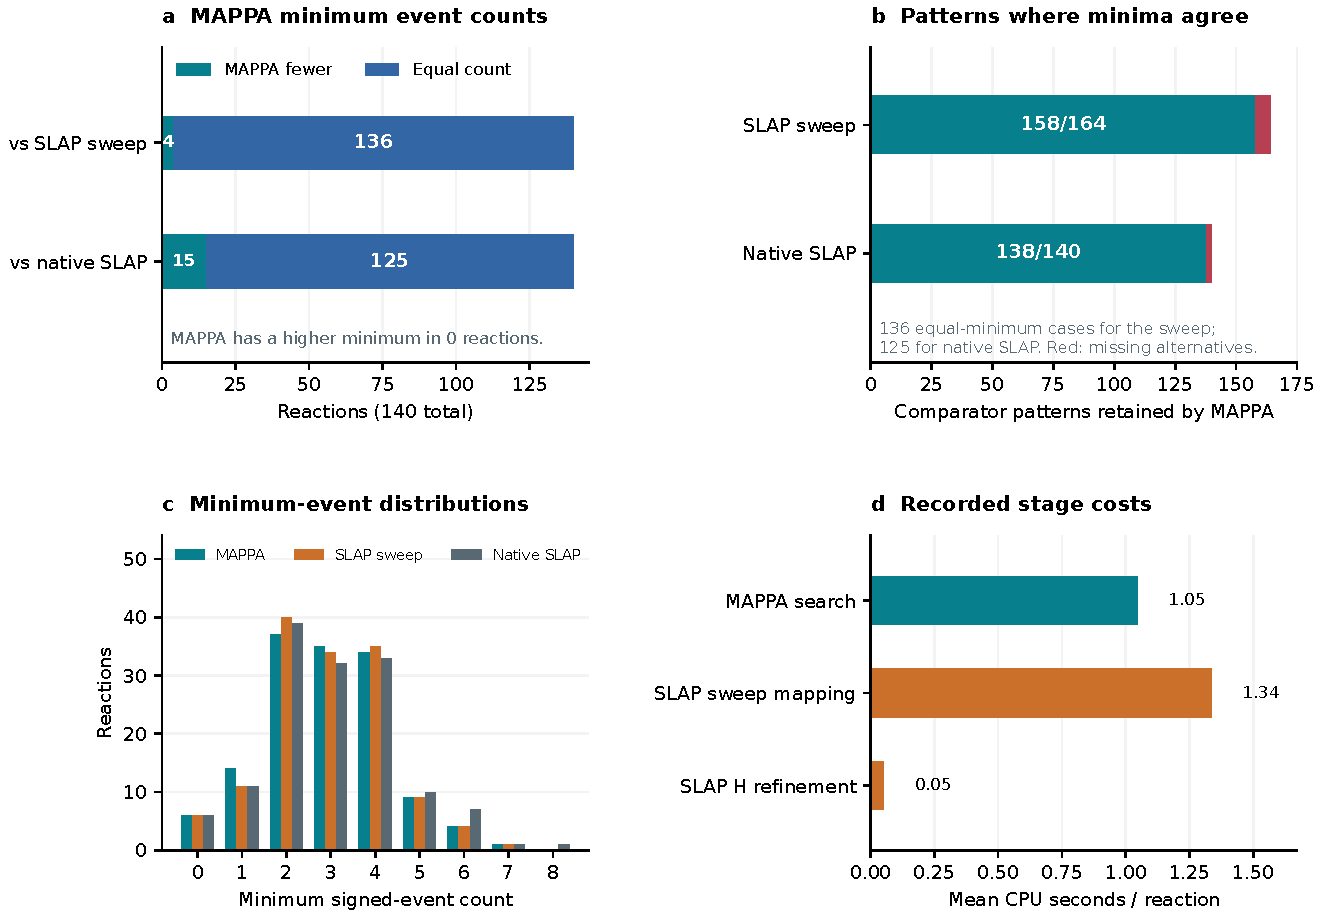
\includegraphics[width=\linewidth]{figs/fig3_coordinate.pdf}
\caption{\textbf{Archived bond-event comparison on 140 coordinate reactions.} MAPPA uses one seed, the sweep, and cap 2,000. (a) Reactions with fewer or equal MAPPA events than each SLAP baseline. (b) Comparator minimum-event patterns recovered by MAPPA at equal minima. (c) Minimum-event count distributions. (d) Mean CPU for search and SLAP refinement, excluding MAPPA decoding (\Cref{tab:coordinate-time}). Atom mappings are unverified; this compares bond events, not mapping accuracy.}
\label{fig:coordinate}
\end{figure}


\FloatBarrier
\subsection{Archived event-window query scope}

For each coordinate reaction, the archived event-window limit was one event above the larger of the native-SLAP and SLAP-sweep minima. All \FlatFamilies{} retained families were exhausted within these limits, without a class-count cap. Higher-event patterns are outside this completeness claim. An event class records the signed atom-pair changes, modulo source permutations preserving every thresholded bond-change test against the opposite endpoint. Each class has a concrete mapping witness. This explicit whole-reaction query is separate from ordinary decoding into shared local fragment responses.

\begin{table}[H]
\centering\small
\caption{\textbf{Archived complete event-window queries on all 140 reactions.} Every retained family is certified within the listed per-case event limit.}
\input{includes/generated-decoder-table}
\end{table}

The query used event invariance to certify constant families and encoded remaining choices in Z3~\citep{demoura2008}. A family was certified by exhaustion, a valid lower bound excluding the window, or unsatisfiability after excluding all discovered classes. An exhausted resource budget remained incomplete. The explicit query adapter can simplify adjacent nested action groups by exact generator-membership checks: if $H\leq G$, then $HG=GH=G$. This adapter simplification is separate from ordinary catalogue reduction in \Cref{sec:reduction-details}. Completeness within an event window concerns the saved families, not exhaustive structural search.

\subsection{Archived Golden nonrecoveries}

\begin{table}[ht]
\centering\small
\caption{\textbf{The eleven archived ten-seed Golden nonrecoveries.} Case indices are zero-based. Retained pair counts cover every terminal in both directions and every saved cut at ten seed orderings and cap 100. The four cardinality mismatches concern exact reference relations, including unmatched atoms. This is not the nonrecovery set of the current one-seed validation.}
\label{tab:golden-misses}
\input{includes/generated-miss-table}
\end{table}

Independent reconstruction agrees with the supplied references in all eleven cases. Four require a different number of matched pairs; seven require correspondences absent from the retained families. All have at least one capped direction, but this does not identify the cap as the cause. The archived uncapped traces below demonstrate greedy-growth exclusions in two cases. Reference-directed feasibility checks are diagnostic and do not contribute to benchmark recovery. Per-case certificates and traces are linked in the repository.

Two archived traces show how greedy extension excluded a representable reference. One reference exchanges adjacent labels in an otherwise unchanged pyridine ring; another exchanges the carbonyl-oxygen attachments of oxalic acid across its retained carbons. Growth preserved bonds that these correspondences require separating. Uncapped trajectories still missed both references, while reference-constrained fragment choices established their representability. In the oxalic-acid example, a reference-selected three-edge relaxation also exposed the reference to matching; the single-edge sweep did not contain that cut set. These are feasibility diagnostics, not additional benchmark recoveries or traces of the current matcher. For the other five correspondence misses, the audit did not isolate cap truncation from unsampled growth choices. They motivate selective alternatives to successful growth extensions and explicit choices about leaving atoms unmatched, rather than treating larger caps or more symmetry expansion as sufficient remedies.

Only one of the eleven misses is recovered by any tested comparator configuration, including the SLAP sweep. The shared failures warrant inspection of the supplied correspondences as well as search improvements; they do not establish annotation errors. All eleven remain in the reported denominator. Independent evaluation on annotated coordinate reactions is needed to assess generalization beyond the development collection.

\subsection{Archived branch-cap and CPU-time ablation on Golden}
\label{sec:cap-ablation}

The archived study ran the twelve configurations in \Cref{tab:golden-caps} on all 1,851 Golden reactions using an AMD EPYC 9J14 CPU. Both search directions are unioned. SLAP unions its binary and weighted modes. Search and reference verification have separate fixed resource budgets. The recorded cap-100 recovery counts reproduce the archived primary evaluation. At cap 2,000, unresolved counts increase with seed count. Among reactions resolved at both caps, no swept configuration gains or loses a reference recovery.

\begin{table}[htbp]
\centering\footnotesize
\caption{\textbf{Archived Golden branch-cap ablation with paired SLAP baselines.} Recovery counts confirmed reference inclusion over all 1,851 records; unknown cases remain in the denominator. CPU values are seconds per reaction. Paired CPU uses the same 1,403 reactions whose searches finish under every configuration. Spent CPU averages recorded search cost over all 1,851 selected attempts, including interrupted calls; it is not completed-search latency. Both timings exclude reference verification and initial imports. Superseded attempts are excluded. Cap 100 with a one-seed sweep is the default setting.}
\label{tab:golden-caps}
\begin{tabular}{lrrr rrr}\toprule
Method & Cap & Seeds & Recovered (\%) & Unknown & Paired CPU & Spent CPU\\\midrule
MAPPA uncut & 100 & 1 & 1,489 (80.44) & 0 & 0.040 & 0.085\\
MAPPA sweep (default) & 100 & 1 & 1,834 (99.08) & 0 & 0.963 & 3.873\\
MAPPA sweep & 100 & 2 & 1,834 (99.08) & 0 & 1.619 & 7.260\\
MAPPA sweep & 100 & 3 & 1,837 (99.24) & 0 & 2.265 & 10.556\\
MAPPA sweep & 100 & 10 & 1,840 (99.41) & 0 & 6.993 & 33.211\\
MAPPA uncut & 2,000 & 1 & 1,508 (81.47) & 5 & 0.086 & 0.517\\
MAPPA sweep & 2,000 & 1 & 1,834 (99.08) & 2 & 4.317 & 30.055\\
MAPPA sweep & 2,000 & 2 & 1,834 (99.08) & 4 & 8.283 & 48.549\\
MAPPA sweep & 2,000 & 3 & 1,837 (99.24) & 6 & 12.201 & 61.890\\
MAPPA sweep & 2,000 & 10 & 1,835 (99.14) & 12 & 43.843 & 113.777\\
SLAP uncut & -- & -- & 1,661 (89.74) & 1 & 0.105 & 0.659\\
SLAP sweep & -- & -- & 1,794 (96.92) & 5 & 2.793 & 9.895\\
\bottomrule\end{tabular}

\end{table}

The ten-seed cap-2,000 run leaves five references recovered at cap 100 unresolved, accounting for its lower confirmed count. The bounded SLAP sweep confirms 1,794 references here, compared with 1,796 in the archived primary evaluation: two previously recovered cases are unresolved under this study's limits. These outcomes are reported separately from verified exclusions. The paired timing cohort excludes 448 reactions because at least one configuration does not finish; the all-attempt cost column exposes the additional computational cost on those difficult reactions. Source pins, individual outcomes, directional costs, and reproduction scripts are provided with the code.



\FloatBarrier
\subsection{Archived end-to-end timing on coordinate reactions}

The archived September implementation completed search and event-window decoding for 140/140 coordinate reactions. On this full set, the full pipeline takes a mean 6.07 CPU seconds per reaction (median 0.81; 95th percentile 25.47). Decoding accounts for a mean 4.65 CPU seconds (median 0.29). These measurements include search, final-family construction, decoding, and candidate output; they are separate from the search-only comparison above (\Cref{tab:end-to-end}).


The historical study measured one-seed, cap-2,000 cut-sweep search followed by its event-window decoder on the Apple M4 Pro CPU. CPU times are reported per reaction. The event thresholds and windows match the bond-event comparison, with no class-count cap. All 140 completed reactions reproduce the archived event-class sets and family counts. Median end-to-end wall time is 0.96 seconds. Timing includes input loading, checkpoint I/O, final-family construction, decoding, and candidate serialization; initial imports and reference-set verification are excluded. All 140 reactions finish within the five-minute watchdog. Detailed timing records and reproduction instructions are provided with the code.


\begin{table}[htbp]
\centering
\caption{\textbf{Archived MAPPA search plus event-window queries.} CPU seconds per completed reaction in the 140-reaction pass. The final row measures the whole pipeline; medians and percentiles of individual stages are not additive. Completion coverage and timing scope are stated above.}
\label{tab:end-to-end}
\begin{tabular}{@{}lrrr@{}}\toprule
Stage & Mean CPU s & Median CPU s & 95th pct. CPU s\\\midrule
MAPPA sweep search & 1.257 & 0.300 & 3.468\\
Final-family catalogue & 0.156 & 0.019 & 0.595\\
Bond-event decoding & 4.647 & 0.288 & 24.361\\
Candidate serialization & 0.005 & 0.001 & 0.015\\
End to end & 6.073 & 0.812 & 25.470\\
\bottomrule\end{tabular}

\end{table}
